\documentclass{beamer}
\usepackage{svg}
\usepackage{wrapfig}
\usetheme{Madrid}
\usepackage{graphicx} % Required for inserting images
\usepackage{listofitems} % for \readlist to create arrays
\usepackage{forest}
\usepackage{caption}
\usepackage{listings}
\usepackage{tikz}
\captionsetup{skip=5pt}
\setbeamertemplate{caption}[numbered]
\usefonttheme{serif}

\definecolor{dgreen}{RGB}{0, 155, 61}
\definecolor{dred}{RGB}{229, 0, 0}
\tikzstyle{mynode}=[thin,draw=black,fill=black!20,circle,minimum size=3pt, inner sep=0pt]

\title[Le jeu Fanorona]{\LARGE Quand l'intelligence artificielle est livrée à elle-même}
\author[Mathis STEINBERGER]{Mathis STEINBERGER\texorpdfstring{\\Eloi de PIERREFEU}{}}

\date[2023-2024]{\scriptsize
\textbf{N°SCEI 12992}
\texorpdfstring{\\Positionnement thématique\\INFORMATIQUE (Informatique pratique)\\INFORMATIQUE (Informatique Théorique)\\MATHEMATIQUES (Géométrie)}{}
}

\newcommand{\svg}[4]{
    \begin{figure}[h]
        \centering
        \includesvg[width = #1]{#2}
        \caption{#3}
        \label{#4}
    \end{figure}
}

\begin{document}
\AtBeginSection[]
{
  \begin{frame}
    \frametitle{Plan}
    \tableofcontents[currentsection]
  \end{frame}
}

\frame{\titlepage}

\begin{frame}{Plan}
    \tableofcontents
\end{frame}

\section{Introduction et présentation du sujet}

\begin{frame}{Définitions des termes du sujet}
    \begin{columns}
        \begin{column}{0.43\textwidth}
        \centering
        \begin{figure}[h]
            \begin{minipage}[b]{\linewidth}
            \centering
                \includesvg[width = 5cm]{images/Fanorona.svg}
                \caption{Fanorona}
                \label{Fig1}
            \end{minipage}
            \vfill
            \begin{minipage}[b]{\linewidth}
            \centering
                \includegraphics[width = 5cm]{images/Fanoronaprises.jpeg}
                \caption{Captures}
                \label{Fig2}
            \end{minipage}
        \end{figure}
    \end{column}
    \begin{column}{0.57\textwidth}
        \begin{itemize}
            \item Jeu combinatoire
            \begin{itemize}
                \item Pas de hasard
                \item Concept de "Position"
                \item Concept de "Coup"
                \item À tour de rôle
                \item But : remplir des "conditions de victoire"
            \end{itemize}
            \item Jeu à informations parfaites
            \begin{itemize}
                \item Informations accessibles par tous
            \end{itemize}
        \end{itemize}
    \end{column}
    \end{columns}
\end{frame}

\begin{frame}{Problèmes posés par le jeu "Fanorona"}
\begin{block}{Particularité}
Possibilité de jouer plusieurs "coups" en un tour
\end{block}
\begin{block}{Contraintes posées par le jeu}
\begin{itemize}
    \item Très peu de publications
    \item Pas de base de données
\end{itemize}
\end{block}
\textbf{Problématique:} Comment créer une intelligence artificielle sans données et sans heuristique efficace pour le Fanorona ?
\end{frame}

\section{Étude théorique}

\begin{frame}{Où en sont les recherches actuelles sur le jeu}
    MAARTEN P. D. SCHADD trouve en 2008 un moyen d'assurer l'égalité. Cette stratégie de décompose en deux parties:
    \begin{block}{Stratégie}
        \begin{itemize}
            \item Se ramener aux états "endgame" avec une recherche pas Nombre de Preuve (PNS)
            \item Finir le travail avec une base de données de coups à jouer pour gagner depuis un état endgame
        \end{itemize}
    \end{block}
    \setbeamercolor{block title}{bg=dgreen,fg=white}
    \setbeamercolor{item}{fg=dgreen}
    \begin{block}{Point fort}
        \begin{itemize}
            \item PNS est très adapté pour ce genre de problème
        \end{itemize}
    \end{block}
    \setbeamercolor{block title}{bg=dred,fg=white}
    \setbeamercolor{item}{fg=dred}
    \begin{block}{Point faible}
        \begin{itemize}
            \item SCHADD explique lui même la difficulté de construire une telle base de données
        \end{itemize}
    \end{block}
\end{frame}

\begin{frame}{La recherche par Nombre de Preuve (PNS)}
    \begin{forest}
    for tree={
    grow=south,
    parent anchor=south,
    child anchor=north,
    align=center,
    l sep=10mm,
    s sep=-6pt,
    inner sep=2pt
  }
  [{\parbox{3cm}{\centering \includegraphics[width=2cm]{images/etats0.jpg}\\ \tiny $P_0=\min(P_1,...,P_5)$\\ $D_0=D_1+...+D_5$}},
    [{\parbox{2.4cm}{\centering \includegraphics[width=2cm]{images/etats1.jpg}\\ \tiny $P_1=P_{1,1}+...$\\ $D_1=\min(D_{1,1},...)$}},
    [\ .\ \ ],[\ .\ \ ],[\ .\ \ ],[\ .\ \ ],,[\ .\ \ ]
    ]
    [{\parbox{2.4cm}{\centering \includegraphics[width=2cm]{images/etats2.jpg}\\ \tiny $P_2=P_{2,1}+...$\\ $D_2=\min(D_{2,1},...)$}},
    [\ .\ \ ],[\ .\ \ ],[\ .\ \ ],[\ .\ \ ],,[\ .\ \ ]
    ]
    [{\parbox{2.4cm}{\centering \includegraphics[width=2cm]{images/etats3.jpg}\\ \tiny $P_3=P_{3,1}+...$\\ $D_3=\min(D_{3,1},...)$}},
    [\ .\ \ ],[\ .\ \ ],[\ .\ \ ],[\ .\ \ ],,[\ .\ \ ]
    ]
    [{\parbox{2.4cm}{\centering \includegraphics[width=2cm]{images/etats4.jpg}\\ \tiny $P_4=P_{4,1}+...$\\ $D_4=\min(D_{4,1},...)$}},
    [\ .\ \ ],[\ .\ \ ],[\ .\ \ ],[\ .\ \ ],,[\ .\ \ ]
    ]
    [{\parbox{2.4cm}{\centering \includegraphics[width=2cm]{images/etats5.jpg}\\ \tiny $P_5=P_{5,1}+...$\\ $D_5=\min(D_{5,1},...)$}},
    [\ .\ \ ],[\ .\ \ ],[\ .\ \ ],[\ .\ \ ],,[\ .\ \ ]
    ]
  ]
\end{forest}
\end{frame}

\begin{frame}{Le Endgame}
    Pourquoi ne pas faire comme le pré-endgame ?
    \setbeamercolor{block title}{bg=dred,fg=white}
    \setbeamercolor{item}{fg=dred}
    \begin{block}{Problème}
    \begin{itemize}
        \item Il y a bien plus d'état accessible au endgame
        \item La seule évaluation possible utile est "Ai-je gagné ?"
    \end{itemize}
    \end{block}
    \begin{block}{Conséquences}
        Un simple élagage $\alpha\beta$ devra être de profondeur bien plus importante, donc l'algorithme mettrai trop de temps à évaluer le score de plateau.
    \end{block}
    \setbeamercolor{block title}{bg=dgreen,fg=white}
    \setbeamercolor{item}{fg=dgreen}
    \begin{block}{Solution proposée}
        Faire ces calculs en amont, afin de ne pas avoir à les faire pendant la partie, par l'utilisation d'un réseau de neurone
    \end{block}
\end{frame}

\begin{frame}{Le Endgame - Réseau de neurone}
    \begin{columns}
    \begin{column}{0.25\textwidth}
        \centering
        \includegraphics[width = 2.5cm]{images/Endgame.png}
    \end{column}
    \begin{column}{0.1\textwidth}
        \centering
        $\longrightarrow$
    \end{column}
    \begin{column}{0.01\textwidth}
        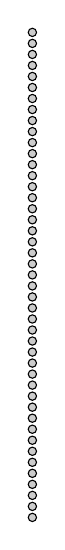
\begin{tikzpicture}[x=.1cm,y=1.4cm]
            \readlist\Nnod{45} % number of nodes per layer
                % \Nnodlen = length of \Nnod (i.e. total number of layers)
                % \Nnod[1] = element (number of nodes) at index 1
                \foreachitem \N \in \Nnod{ % loop over layers
                % \N     = current element in this iteration (i.e. number of nodes for this layer)
                % \Ncnt  = index of current layer in this iteration
                    \foreach \i [evaluate={\x=\Ncnt; \y=\N/2-(\i)+0.5; \prev=int(\Ncnt-1);}] in {1,...,\N}{ % loop over nodes
                            \node[mynode] (N\Ncnt-\i) at (\x,\y/10) {};
                            \ifnum\Ncnt>1 % connect to previous layer
                            \foreach \j in {1,...,\Nnod[\prev]}{ % loop over nodes in previous layer
                                \draw[ultra thin] (N\prev-\j) -- (N\Ncnt-\i); % connect arrows directly
                            }
                            \fi % else: nothing to connect first layer
                    }
                }
        \end{tikzpicture}
    \end{column}
    \begin{column}{0.1\textwidth}
        \centering
        $\longrightarrow$
    \end{column}
    \begin{column}{0.4\textwidth}
        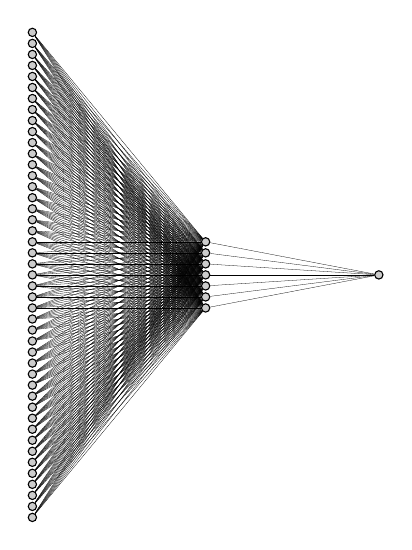
\begin{tikzpicture}[x=2.2cm,y=1.4cm]
            \readlist\Nnod{45,7,1} % number of nodes per layer
                % \Nnodlen = length of \Nnod (i.e. total number of layers)
                % \Nnod[1] = element (number of nodes) at index 1
                \foreachitem \N \in \Nnod{ % loop over layers
                % \N     = current element in this iteration (i.e. number of nodes for this layer)
                % \Ncnt  = index of current layer in this iteration
                    \foreach \i [evaluate={\x=\Ncnt; \y=\N/2-(\i)+0.5; \prev=int(\Ncnt-1);}] in {1,...,\N}{ % loop over nodes
                            \ifnum\i=1 \fi
                            \node[mynode] (N\Ncnt-\i) at (\x,\y/10) {};
                            \ifnum\Ncnt>1 % connect to previous layer
                            \foreach \j in {1,...,\Nnod[\prev]}{ % loop over nodes in previous layer
                                \draw[ultra thin] (N\prev-\j) -- (N\Ncnt-\i); % connect arrows directly
                            }
                            \fi % else: nothing to connect first layer
                    }
                }
        \end{tikzpicture}
    \end{column}
    \begin{column}{0.1\textwidth}
        \centering
        $\longrightarrow$
    \end{column}
    \begin{column}{0.05\textwidth}
        \centering
        \scriptsize $0.02$
    \end{column}
    \end{columns}
\end{frame}

\section{Implémentation du jeu et de l'IA}

\begin{frame}{Implémentation du jeu}
    \begin{columns}
        \begin{column}{0.5\textwidth}
            \begin{figure}
                \centering
                \includegraphics[width = 5cm]{images/etats0.jpg}
                \caption{Pièces jouables}
                \label{fig:Playable-pieces}
            \end{figure}
        \end{column}
        \begin{column}{0.5\textwidth}
            \begin{figure}
                \centering
                \includegraphics[width = 5cm]{images/fleche.png}
                \caption{Mouvement(s) possible(s)}
                \label{fig:Fleches}
            \end{figure}
        \end{column}
    \end{columns}
    \begin{block}{Contrainte UTF-8}
        Pas d'implémentation des intersections
    \end{block}
\end{frame}

\begin{frame}{Préparation des données}
\scriptsize Création de la fonction : \texorpdfstring{\\}{} {\fontfamily{cmtt}\selectfont 
\scriptsize board* flatten\_possibilities(board gameboard, int color, int* len, bool endgame)%
}
\begin{columns}
    \begin{column}{0.45\textwidth}
        \begin{forest}
    for tree={
    grow=south,
    parent anchor=south,
    child anchor=north,
    align=center,
    l sep=10mm,
    s sep=-6pt,
    inner sep=2pt
  }
  [{\parbox{3cm}{\centering \includegraphics[width=2cm]{images/iniflat.png}}},
    [{\parbox{2.4cm}{\centering \includegraphics[width=2cm]{images/flat1.png}}}]
    [{\parbox{2.4cm}{\centering \includegraphics[width=2cm]{images/flat2.png}}},
        [{\parbox{2.4cm}{\centering \includegraphics[width=2cm]{images/flat3.png}}}]
    ]
  ]
\end{forest}
    \end{column}
    \begin{column}{0.05\textwidth}
        $\longrightarrow$
    \end{column}
    \begin{column}{0.50\textwidth}
    \centering
        \Bigg[ \raisebox{-0.45\height}{\includegraphics[width=1.5cm]{images/flat1.png}},
        \raisebox{-0.45\height}{\includegraphics[width=1.5cm]{images/flat2.png}},
        \raisebox{-0.45\height}{\includegraphics[width=1.5cm]{images/flat3.png}} \Bigg]
    \end{column}
\end{columns}
\end{frame}

\begin{frame}{Implémentation de l'IA - Pré-Endgame}
    \begin{block}{Rappel de la théorie}
        \begin{itemize}
            \item On explore l'arbre des états jusqu’à tomber sur un état endgame
        \end{itemize}
    \end{block}
    \setbeamercolor{block title}{bg=dgreen,fg=white}
    \setbeamercolor{item}{fg=dgreen}
    \begin{block}{En pratique, un $\alpha\beta$ sera utilisé}
    \begin{itemize}
        \item Bien moins d'optimisations nécéssaires
        \item Plus efficace si l'on cherche a créer une IA
    \end{itemize}
    \end{block}
    \setbeamercolor{block title}{bg=black, fg=white}
    \begin{block}{Pseudo-Heuristique H utilisée}
        Pour un état P du plateau: $H(P)=\dfrac{|P|_{\text{Alliées}}}{|P|_{\text{Adverses}}}$ 
    \end{block}
\end{frame}

\begin{frame}{Implémentation de l'IA - Endgame}
    \begin{block}{Informations générales:}
        \begin{itemize}
        \item Taille de l'entrée : 45 neurones
        \item Taille de la couche cachée : 7 neurones
        \item Taille de la couche de sortie : 1 neurone
    \end{itemize}
    \end{block}
    \setbeamercolor{block title}{bg = black, fg = white}
    \setbeamercolor{item}{fg = black}
    \begin{block}{Informations techniques:}
        \begin{itemize}
        \item Fonction d'activation : sigmoid
        \item Fonction de perte : Moindres Carrées
        \item Taux d'apprentissage : $10^{-5}$
    \end{itemize}
    \end{block}
    Où sigmoid est la fonction $s:x\mapsto \dfrac{1}{1+e^{-x}}$
\end{frame}

\begin{frame}{Résultats}
\setbeamercolor{block title}{bg=black,fg=white}
    \setbeamercolor{item}{fg=black}
    \begin{block}{Résultats du Pré-Endgame avec $\alpha\beta$}
        \begin{columns}
            \begin{column}{0.4\textwidth}
                \vspace{+1.6em}
                \centering
                \small Contre l'IA de y8.com :
            \end{column}
            \begin{column}{0.3\textwidth}
                \begin{minipage}[t]{\textwidth}
                \centering
                \begin{figure}
                    \centering
                    \includegraphics[width=3cm]{images/JouerPremier.jpg}
                    \caption{\small L'IA en $1^{\text{ere}}$}
                    \label{fig:enter-label}
                \end{figure}
                \end{minipage}
            \end{column}
            \begin{column}{0.3\textwidth}
                \begin{minipage}[t]{\textwidth}
                \centering
                \begin{figure}
                    \centering
                    \includegraphics[width=3cm]{images/JouerDeuxieme.jpg}
                    \caption{\small L'IA en $2^\text{e}$}
                \end{figure}
                \end{minipage}
            \end{column}
        \end{columns}
    \end{block}
    \begin{block}{Résultats Finaux}
        \resizebox{\textwidth}{!}{%
    \begin{tabular}{|*{10}{c|}}
    \hline
     IA  &  $\alpha\beta$ + HR (B)  & Adversaire (N)  & $\alpha\beta$ + HR (N)  & Adversaire (B) \\
    \hline
     y8.com  & 100\%  & 0\%  & 100\%  & 0\% \\
    \hline
     Conqueror (Microsoft)  & 100\%  & 0\%  & 100\% & 0\% \\
    \hline
     Domination (Microsoft)  & 100\%  & 0\%  & 90\% & 10\% \\
     \hline
     Tournament (Microsoft) & 60\% & 40\% & 40\% & 60\% \\
    \hline
     $\alpha\beta$ + HR  & 57\% & 43\% & &\\
     \hline
\end{tabular}}
    \end{block}
\end{frame}

\section{Comparaison avec les résultats sur le jeu de HEX}

\begin{frame}{Comparaison avec les résultats sur le jeu de HEX}
    
\end{frame}

\section{Conclusion et discussions}

\begin{frame}{Conclusion et discussions}
    La technique d'heurstique à fait ses preuves, mais la solution présentée n'est pas parfaite
    \begin{block}{Pistes d'améliorations possibles}
        \begin{itemize}
            \item Changer le type de réseau de neurone
            \item Accélérer l'entrainement de l'heuristique
            \item Entraîner l'heuristique plus longtemps
            \item Augmenter la profondeur de recherche pour le Pré-Endgame ou le Endgame
        \end{itemize}
    \end{block}
    On peut néanmoins appliquer ces principe pour des tailles et dimensions supérieures du plateau.
\end{frame}

\end{document}

%{\parbox{3cm}{\centering \footnotesize Initial \\ \includegraphics[width=2cm]{images/etats0.jpg}}}
%$P_1=\min(P_{1,1},...,P_{1,|A_1|})$ \\ $D_1=D_6+...+D_5$